\section{Results}
\label{sec:results}
\begin{table}[t]
\centering
\caption{Measured Data Audit and Partition for the OpSpam v1.4 Corpus}
\label{tab:data}
\footnotesize
\begin{tabular}{@{}p{0.52\columnwidth}p{0.40\columnwidth}@{}}
\toprule
Item & Value \\
\midrule
Reviews retained / removed & 1,600 / 0 \\
Truthful / deceptive & 800 / 800 \\
Hotels; reviews per hotel & 20; 80 (40 per class) \\
Exact duplicate pairs (excess copies) & 4 (4), all truthful negative \\
Further near-duplicate pairs & 0 (Jaccard $\ge$ 0.80) \\
Reviewer ID / rating / date available & No / No / No \\
Uncompressed text & 1,290,226 bytes \\
Seed-42 train / validation / test & 1,120 / 240 / 240 \\
Seed-42 hotels (train / val / test) & 14 / 3 / 3 \\
Seed-42 test hotels & Conrad, James, Knickerbocker \\
Class balance in every partition & 50\% deceptive \\
\bottomrule
\end{tabular}
\end{table}

\begin{table*}[t]
\centering
\caption{Predictive Performance on Hotel-Disjoint Test Data. Seed 42 is the primary 240-review test set (three hotels); the 5-fold row pools out-of-fold predictions for all 1,600 reviews (20 hotels). Class 1 = deceptive; threshold 0.5.}
\label{tab:main}
\footnotesize
\begin{tabular}{@{}llccccccc@{}}
\toprule
Evaluation & Model & Accuracy & Precision$_1$ & Recall$_1$ & F1$_1$ & Macro-F1 & AP & ROC-AUC \\
\midrule
Seed 42 test ($n=240$) & TF--IDF + LR & 0.8917 & \textbf{0.8790} & 0.9083 & 0.8934 & 0.8916 & 0.9539 & 0.9527 \\
 & RoBERTa-base & \textbf{0.9000} & 0.8380 & \textbf{0.9917} & \textbf{0.9084} & \textbf{0.8992} & \textbf{0.9864} & \textbf{0.9852} \\
\addlinespace
Grouped 5-fold CV ($n=1{,}600$) & TF--IDF + LR & 0.8794 & \textbf{0.9020} & 0.8512 & 0.8759 & 0.8793 & 0.9504 & 0.9469 \\
 & RoBERTa-base & \textbf{0.8925} & 0.8576 & \textbf{0.9413} & \textbf{0.8975} & \textbf{0.8922} & \textbf{0.9648} & \textbf{0.9638} \\
\bottomrule
\end{tabular}
\end{table*}


\subsection{Data and Partitions}
Table~\ref{tab:data} summarises the audited corpus. The four exact-duplicate pairs (one each at Monaco and Affinia, two at Omni) are truthful negative reviews with consistent labels; the near-duplicate screen found no further pairs. Since every hotel contributes 80 reviews, the hotel components produce identical partition sizes for all three seeds (1,120/240/240), and each partition is exactly balanced. Seed 42 holds out Conrad, James and Knickerbocker; seed 123 holds out Knickerbocker, Palmer and Swissotel; seed 2026 holds out Amalfi, Monaco and Talbott. No hotel or duplicate group crosses partitions. The LR results reproduce the values reported for the Assignment~3 pilot to four decimal places, which confirms that the rebuilt pipeline implements the same partition and model.

\subsection{RQ1: RoBERTa versus the TF--IDF Baseline}
Table~\ref{tab:main} reports the main comparison. On the primary seed-42 test set, RoBERTa reached a macro-F1 of 0.8992 against 0.8916 for LR, a difference of $+$0.0075. The paired hotel-bootstrap interval for this difference, [$-$0.0143, 0.0252], includes zero, and the prespecified hotel-level randomisation test gave $p=0.742$. The exploratory review-level test, which does not suffer from the three-hotel floor, gave $p=0.864$. The two models disagree on only 34 of the 240 test reviews: 18 are correct only for RoBERTa, 16 only for LR, and 8 reviews defeat both. The grouped cross-validation, in which each of the 20 hotels is tested once, gives the same picture with more data: pooled macro-F1 was 0.8922 for RoBERTa and 0.8793 for LR ($\Delta=+0.0130$, 95\% CI [$-$0.0107, 0.0349], hotel-level $p=0.326$). The answer to RQ1 is therefore negative at the prespecified level: RoBERTa's macro-F1 is not significantly higher than the baseline's.

The two models nevertheless behave differently. RoBERTa ranks reviews better: its AP was 0.9864 against 0.9539, and its ROC-AUC 0.9852 against 0.9527 on the seed-42 test set, and both measures were also higher in cross-validation. Fig.~\ref{fig:pr} shows that the RoBERTa precision--recall curve lies above the LR curve over most of the recall range. At the fixed 0.5 threshold, however, RoBERTa labels too many reviews as deceptive. It missed only one deceptive review but flagged 23 truthful ones, whereas LR missed 11 and flagged 15 (Fig.~\ref{fig:cm}). Its deceptive-class recall was 0.9917 and its precision 0.8380; LR was more balanced (0.9083 and 0.8790). The ranking advantage thus does not translate into a higher macro-F1 because the untuned threshold is poorly placed for RoBERTa's scores.

\begin{figure}[t]\centering
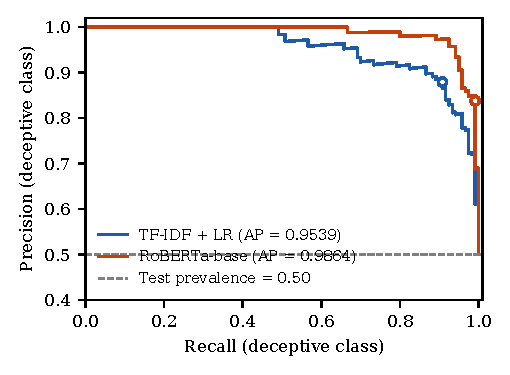
\includegraphics[width=\columnwidth]{figures/precision_recall.pdf}
\caption{Precision--recall curves on the seed-42 test set (240 reviews, three held-out hotels). Open markers show the fixed 0.5 threshold; the dashed line is the test prevalence.}
\label{fig:pr}
\end{figure}

\begin{figure}[t]\centering
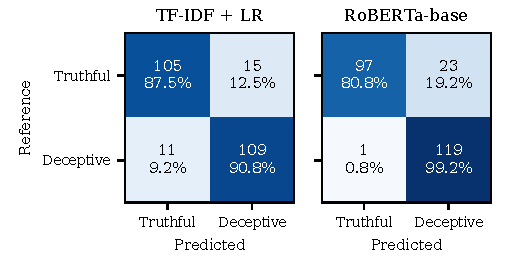
\includegraphics[width=\columnwidth]{figures/confusion_matrix.pdf}
\caption{Seed-42 confusion matrices with counts and row percentages. RoBERTa misses one deceptive review but flags 23 truthful reviews; LR misses 11 and flags 15.}
\label{fig:cm}
\end{figure}

\subsection{RQ2: Stability and Robustness}
Table~\ref{tab:reliability} shows that the small seed-42 advantage does not survive a change of partition. RoBERTa was slightly worse than LR for seed 123 ($-$0.0167) and seed 2026 ($-$0.0019), so the mean difference over the three partitions was $-$0.0037. Partition-to-partition variation (SD 0.0187 for LR and 0.0157 for RoBERTa) is larger than any of the between-model differences, so the choice of test hotels matters more than the choice of model. Validation scores were equally variable: RoBERTa's best validation macro-F1 was 0.9292, 0.8694 and 0.8114 for the three seeds, with the third epoch selected twice and the second once.

Fig.~\ref{fig:hotels} shows the per-hotel out-of-fold results. RoBERTa scored higher for 11 hotels and LR for 9. The largest gains for RoBERTa were at InterContinental (0.8623 to 0.9625), Swissotel (0.8496 to 0.9374) and Sofitel (0.7625 to 0.8599); the largest losses were at Fairmont (0.9500 to 0.8344) and Allegro (0.9250 to 0.8620). The two models therefore fail on different hotels, which explains why their pooled scores are similar while individual reviews are classified differently. By polarity, RoBERTa was stronger on positive reviews (cross-validated macro-F1 0.9237 versus 0.8812) and weaker on negative reviews (0.8604 versus 0.8773), where it produced 87 false positives against 34 for LR.

\begin{figure}[t]\centering
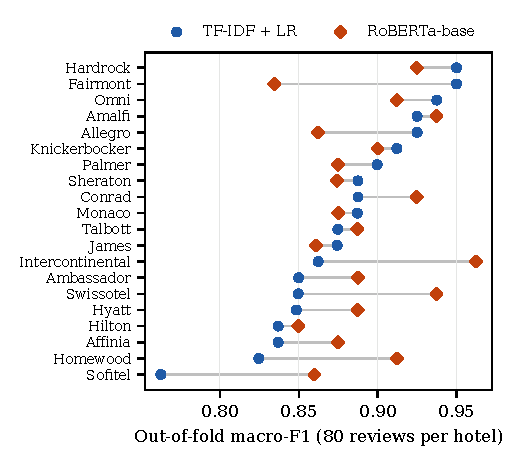
\includegraphics[width=\columnwidth]{figures/per_hotel_cv.pdf}
\caption{Out-of-fold macro-F1 for each of the 20 hotels in the grouped 5-fold cross-validation (80 reviews per hotel), sorted by the LR score. Grey lines connect the two models for the same hotel.}
\label{fig:hotels}
\end{figure}

The formatting perturbations separated the models sharply. LR was unaffected by all three: no prediction changed, because lowercasing and word tokenisation remove these differences. RoBERTa's macro-F1 fell by 0.3261 under uppercasing (95\% CI [$-$0.3988, $-$0.2719]), with 109 of 240 predictions changed and only 13.8\% of reviews still labelled deceptive. Under the whitespace perturbation it fell by 0.5658 and every review was labelled truthful. The tokeniser explains most of this. RoBERTa is case-sensitive, and uppercase text is split into different and more numerous subword tokens, raising the median review length from 158 to 246 tokens. The whitespace perturbation raised the median length to 676 tokens, so 97.1\% of reviews exceeded the 256-token limit and lost most of their content to truncation, compared with 21.2\% of clean reviews. These perturbations do not change the meaning of a review, yet they move RoBERTa far outside its training distribution. The answer to RQ2 is that both models are equally stable across partitions and hotels in aggregate, but RoBERTa is much less robust to surface formatting.

\begin{table}[t]
\centering
\caption{Paired Comparison, Stability and Robustness (Macro-F1). $\Delta$ = RoBERTa minus LR. Bootstrap intervals resample test hotels (2,000 replicates, seed 42).}
\label{tab:reliability}
\scriptsize
\setlength{\tabcolsep}{3pt}
\begin{tabular}{@{}lccc@{}}
\toprule
Quantity & LR & RoBERTa & $\Delta$ \\
\midrule
Seed 42 test & 0.8916 & 0.8992 & $+$0.0075 \\
Seed 123 test & 0.9082 & 0.8915 & $-$0.0167 \\
Seed 2026 test & 0.8708 & 0.8689 & $-$0.0019 \\
Mean (SD) over seeds & 0.8902 (0.0187) & 0.8865 (0.0157) & $-$0.0037 \\
\addlinespace
Seed 42 95\% CI & [0.8492, 0.9373] & [0.8607, 0.9624] & [$-$0.0143, 0.0252] \\
Seed 42 $p$, hotel swap & \multicolumn{3}{r}{0.742} \\
Seed 42 $p$, review swap$^\dagger$ & \multicolumn{3}{r}{0.864} \\
\addlinespace
5-fold 95\% CI & [0.8593, 0.8987] & [0.8791, 0.9067] & [$-$0.0107, 0.0349] \\
5-fold $p$, hotel swap$^\dagger$ & \multicolumn{3}{r}{0.326} \\
Hotels won (of 20) & 9 & 11 & -- \\
\addlinespace
Uppercase, $\Delta$ vs.\ clean & 0.0000 & $-$0.3261 & -- \\
Whitespace, $\Delta$ vs.\ clean & 0.0000 & $-$0.5658 & -- \\
Both, $\Delta$ vs.\ clean & 0.0000 & $-$0.5658 & -- \\
Predictions changed (of 240) & 0 / 0 / 0 & 109 / 142 / 142 & -- \\
\bottomrule
\multicolumn{4}{@{}l}{$^\dagger$Exploratory analysis added after the protocol.}
\end{tabular}
\end{table}


\subsection{What the Baseline Relies On}
The robustness of LR raises the question of which cues it uses. Table~\ref{tab:features} lists the twelve $n$-grams with the largest positive and negative weights in the seed-42 model. Deceptive reviews are signalled by first-person and narrative language (\emph{my}, \emph{my stay}, \emph{my husband}, \emph{recently}, \emph{experience}) and by generic references to the city and hotel (\emph{chicago}, \emph{chicago hotel}, \emph{luxury}). Truthful reviews are signalled by concrete spatial and practical detail (\emph{location}, \emph{floor}, \emph{on}, \emph{bathroom}, \emph{breakfast}, \emph{large}) and by local street and landmark names (\emph{michigan}, \emph{ave}, \emph{river}). This matches the original corpus analysis, in which truthful reviews were more specific about spatial configuration and deceptive reviews used more first-person singular language \cite{ref22,ott2013}. Because these cues are lexical and case-insensitive, the baseline is unaffected by formatting; because many of them describe the writing task (an imagined stay in Chicago) rather than deception in general, they may transfer poorly to commercial fake reviews written by people who know the property.

\begin{table}[t]
\centering
\caption{Twelve Strongest $n$-Gram Weights of the Seed-42 TF--IDF + LR Model. Positive weights favour the deceptive class.}
\label{tab:features}
\footnotesize
\begin{tabular}{@{}lr@{\hspace{1.2em}}lr@{}}
\toprule
Deceptive & Weight & Truthful & Weight \\
\midrule
chicago & 2.33 & location & $-$1.63 \\
my & 1.89 & floor & $-$1.22 \\
luxury & 1.23 & we & $-$1.12 \\
chicago hotel & 1.11 & on & $-$1.10 \\
experience & 1.03 & great & $-$1.05 \\
my stay & 0.99 & michigan & $-$1.02 \\
be & 0.90 & large & $-$0.94 \\
at the & 0.88 & no & $-$0.87 \\
recently & 0.87 & river & $-$0.86 \\
husband and & 0.87 & ave & $-$0.85 \\
my husband & 0.86 & bathroom & $-$0.85 \\
husband & 0.86 & breakfast & $-$0.84 \\
\bottomrule
\end{tabular}
\end{table}

\subsection{RQ3: Computational Cost}
\begin{table}[t]
\centering
\caption{Measured Computational Cost (Seed 42). Throughput: median (range) of five timed passes over the 240 test reviews in batches of 32 after a 100-review warm-up.}
\label{tab:cost}
\footnotesize
\begin{tabular}{@{}lcc@{}}
\toprule
Measure & TF--IDF + LR & RoBERTa-base \\
\midrule
Hardware & Laptop CPU & RTX 4060 Laptop GPU \\
Model size & 12,116 features & 124.6\,M parameters \\
Training time & 0.19\,s & 91.4\,s \\
Peak GPU memory & -- & 4.1\,GB \\
Throughput (reviews/s) & 8,591 (8,322--8,718) & 132.8 (132.8--133.2) \\
Test macro-F1 & 0.8916 & 0.8992 \\
\bottomrule
\end{tabular}
\end{table}

Table~\ref{tab:cost} summarises the cost of each model. The LR baseline fitted in 0.19\,s on the laptop CPU and classified a median of 8,591 reviews per second (range 8,322--8,718 over five passes). RoBERTa required 91.4\,s of GPU fine-tuning for seed 42 (91.4--91.9\,s across seeds) with a peak of 4.1\,GB of GPU memory (5.5\,GB for the other seeds), and classified a median of 132.8 reviews per second on the GPU (range 132.8--133.2). Training was thus about 480 times slower and inference about 65 times slower than for LR, which used no GPU. The complete experiment, including eight RoBERTa fine-tuning runs, took 12.6 minutes. Answering RQ3, the transformer's cost is two orders of magnitude higher, while its macro-F1 gain is not statistically distinguishable from zero.

\subsection{Discussion}
The results qualify the high transformer scores reported on this corpus. Mohawesh et al.\ report 96.03\% accuracy on OpSpam with a RoBERTa--LSTM model \cite{ref15}, whereas RoBERTa-base reached 89.25\% accuracy here under hotel-disjoint cross-validation, close to the near-90\% reported for $n$-gram models by Ott et al.\ \cite{ref22}. Differences in architecture, tuning and partitioning all contribute, so the comparison is indicative rather than direct; the controlled comparison in this study shows that, with partitions and settings held fixed, a well-specified linear model matches the transformer in macro-F1. This mirrors the case study of Kapoor and Narayanan, in which complex models no longer outperformed logistic regression once evaluation errors were corrected \cite{kapoor2023}. The transformer's higher AP and ROC-AUC suggest that its representations do carry additional signal, but extracting it would require calibrating the decision threshold on validation data, which the protocol deliberately did not do. The perturbation results add a practical warning: a detector deployed on reviews that differ in formatting from its training data can fail completely without any change in content, which matters for platforms where text is pasted, reformatted or deliberately obfuscated.
